\section{Demonstration of fitting by DCC models}

\newcommand{\fitScatLength}{-1.05 \pm 0.12 (fit.) \pm +0.09 (syst.) + [ 0.86 \pm 0.15 (fit.) ^{+0.07} _{-0.08} (syst.)]i}
\newcommand{\fitEffRange}{-0.22 \pm 0.40 (fit.) ^{+0.05} _{-0.06} (syst.) + [ -0.42 \pm 0.16 (fit.) ^{+0.12} _{-0.08} (syst.)]i}
\newcommand{\fitPole}{1418.3 ^{+7.5} _{-2.4} (fit.)^{+0.9}_{-1.1} (syst.)}
\newcommand{\fitWidth}{-27.8^{+9.5}_{-0.9} (fit.)^{+1.9}_{-2.1} (syst.)}

\newcommand{\fitAscaleIz}{0.562 \pm 0.015}
\newcommand{\fitAscaleIo}{1.070 \pm 0.040}
\newcommand{\fitAscaleIzVal}{0.562}
\newcommand{\fitAscaleIzErr}{0.015}
\newcommand{\fitAscaleIoVal}{1.070}
\newcommand{\fitAscaleIoErr}{0.040}
\newcommand{\fitAscaleChi}{691/42}
\newcommand{\fitAscaleChiNum}{16.4}

\newcommand{\fitBscaleIz}{0.721 \pm 0.016}
\newcommand{\fitBscaleIo}{1.423 \pm 0.055}
\newcommand{\fitBscaleIzVal}{0.721}
\newcommand{\fitBscaleIoVal}{1.423}
\newcommand{\fitBscaleIzErr}{0.016}
\newcommand{\fitBscaleIoErr}{0.055}
\newcommand{\fitBscaleChi}{220/42}
\newcommand{\fitBscaleChiNum}{5.25}

\newcommand{\fitBBChi}{187/41}
\newcommand{\fitBBChiNum}{4.56}
\newcommand{\fitBBIz}{0.686 \pm 0.017}
\newcommand{\fitBBIo}{1.462 \pm 0.059}
\newcommand{\fitBBphase}{0.828 \pm 0.030}
\newcommand{\fitBBIzVal}{0.686}
\newcommand{\fitBBIoVal}{1.462}
\newcommand{\fitBBphaseVal}{0.828}
\newcommand{\fitBBIzErr}{0.017}
\newcommand{\fitBBIoErr}{0.059}
\newcommand{\fitBBphaseErr}{0.030}
\newcommand{\fitBBDegree}{34.1^{+3.0}_{-3.2}}

\newcommand{\fitBChi}{184/41}
\newcommand{\fitBChiNum}{4.48}
\newcommand{\fitBIz}{0.682 \pm 0.017}
\newcommand{\fitBIo}{1.570 \pm 0.058}
\newcommand{\fitBphase}{0.811 \pm 0.030}
\newcommand{\fitBIzVal}{0.682}
\newcommand{\fitBIoVal}{1.570}
\newcommand{\fitBphaseVal}{0.811}
\newcommand{\fitBIzErr}{0.017}
\newcommand{\fitBIoErr}{0.058}
\newcommand{\fitBphaseErr}{0.030}
\newcommand{\fitBDegree}{35.8^{+2.8}_{-3.1}}

\newcommand{\fitScaleKN}{0.0372 \pm 0.0047}
\newcommand{\fitAreKN}{-1.05 \pm 0.12}
\newcommand{\fitAimKN}{ 0.86 \pm 0.15}
\newcommand{\fitRreKN}{-0.22 \pm 0.40}
\newcommand{\fitRimKN}{ 0.42 \pm 0.16}
\newcommand{\fitKNMass}{1418.3}
\newcommand{\fitKNWidth}{27.8}

\newcommand{\fitScaleKmp}{0.0377 \pm 0.0042}
\newcommand{\fitAreKmp}{-0.95 \pm 0.11}
\newcommand{\fitAimKmp}{ 0.94 \pm 0.16}
\newcommand{\fitRreKmp}{-0.27 \pm 0.40}
\newcommand{\fitRimKmp}{ 0.52 \pm 0.18}
\newcommand{\fitKmpMass}{1417.6}
\newcommand{\fitKmpWidth}{30.3}

\newcommand{\fitScaleKzeroN}{0.0367 \pm 0.0053}
\newcommand{\fitAreKzeroN}{-1.13 \pm 0.13}
\newcommand{\fitAimKzeroN}{ 0.79 \pm 0.15}
\newcommand{\fitRreKzeroN}{-0.16 \pm 0.40}
\newcommand{\fitRimKzeroN}{ 0.33 \pm 0.16}
\newcommand{\fitKzeroNMass}{1419.3}
\newcommand{\fitKzeroNWidth}{25.9}



Next, we performed demonstration of fitting by DCC models to discuss each component how to contribute each spectra.
First, we use the strength of $I=0$ and $I=1$ as free parameter, which scale $I=0$ and $I=1$ spectra.
The interferance term also change corespond to the isospin relation  as follow rrepresentation.

\begin{eqnarray}
  & & \frac{d\sigma_{\pi^-\Sigma^+}}{dM d\Omega}
  = \frac{1}{3} A_{I=0} |T_{I=0}|^2 + \frac{1}{2} A_{I=1} |T_{I=1}|^2 + \frac{2}{\sqrt{6}} \sqrt{A_{I=0} A_{I=1}} \mbox{\bf Re}(T_{I=0}T_{I=1}^*) \nonumber \\
  & & \frac{d\sigma_{\pi^+\Sigma^-}}{dM d\Omega}
  = \frac{1}{3} A_{I=0} |T_{I=0}|^2 + \frac{1}{2} A_{I=1} |T_{I=1}|^2 - \frac{2}{\sqrt{6}} \sqrt{A_{I=0} A_{I=1}} \mbox{\bf Re}(T_{I=0}T_{I=1}^*) \nonumber \\
  & & \frac{d\sigma_{\pi^0\Sigma^-}}{dM d\Omega}  =  \frac{1}{2} A_{I=1} |T_{I=1}|^2 \nonumber \\
  \label{eq::CS_iso_wA}
\end{eqnarray}


Where, $A_{I=0}$ and $A_{I=1}$ is scaling factor introduced as 2-step scattering strength.
And interference term is changed according to square root of each strength.

Fig.[\ref{fig:fit_A_scale}] shows about fitting result of Model.A,
in which above figures show obtained spectra and bottom figures show calculated spectra.
We note that fitting are used only above 3 spectra.
At the result, we obtain $A_{I=0}=\fitAscaleIz$ and $A_{I=1}=\fitAscaleIo$ with $\chi^2/NDF=\fitAscaleChi \sim \fitAscaleChiNum$.
In the model.A, $\pi^-\Sigma^0$ of $I=1$ is obtained good matched, that strongly affect above the threshold, but I=0 below the threshold is not matched.
Therefore, the model.A can not explained obtained spectra, as the  shown Fig.[\ref{fig:fit_A_scale}].

\begin{figure}[htbp]
  \begin{tabular}{cc}
    \begin{minipage}{0.5\hsize}
      \centering
      \includegraphics[width=6.0cm]{../pic/Dron/fit_model_A_fix_Phi/I0_fit.eps}
    \end{minipage}

    \begin{minipage}{0.5\hsize}
      \centering
      \includegraphics[width=6.0cm]{../pic/Dron/fit_model_A_fix_Phi/pimS0_fit.eps}
    \end{minipage}
  \end{tabular}

  \centering
  \includegraphics[width=6.0cm]{../pic/Dron/fit_model_A_fix_Phi/interfer_fit.eps}
  \caption{
    These figures show the fitting of parametric strengths of $I=0$ and $I=1$ using Model.A.
    The notation is the same as in Fig.\ref{fig:decomposed_DCC}.
    Only the red line representing Model.A (red line) is plotted.
  }
  \label{fig:fit_A_scale}
\end{figure}

\begin{figure}[htbp]
  \begin{tabular}{cc}
    \begin{minipage}{0.5\hsize}
      \centering
      \includegraphics[width=6.0cm]{../pic/Dron/fit_model_B_fix_Phi/I0_fit.eps}
    \end{minipage}

    \begin{minipage}{0.5\hsize}
      \centering
      \includegraphics[width=6.0cm]{../pic/Dron/fit_model_B_fix_Phi/pimS0_fit.eps}
    \end{minipage}
  \end{tabular}

  \centering
  \includegraphics[width=6.0cm]{../pic/Dron/fit_model_B_fix_Phi/interfer_fit.eps}
  \caption{
    This figure presents the results of fitting the experimental data using Model B.
    The blue line represents the fit results, while other notations follow the same conventions as in Figure \ref{fig:fit_A_scale}.
  }
  \label{fig:fit_B_scale}
\end{figure}


\begin{figure}
  \centering
  \begin{tabular}{ccc}
    \begin{minipage}{0.330\hsize}
      \centering
      $\pi^-\Sigma^+$ mode
      \includegraphics[width=4.5cm]{../pic/Dron/fit_model_B_2/pimSp_fit.eps}
    \end{minipage}

    \begin{minipage}{0.33\hsize}
      \centering
      $\pi^+\Sigma^-$ mode
      \includegraphics[width=4.5cm]{../pic/Dron/fit_model_B_2/pipSm_fit.eps}
    \end{minipage}

    \begin{minipage}{0.33\hsize}
      \centering
      $\pi^-\Sigma^0$ mode
      \includegraphics[width=4.5cm]{../pic/Dron/fit_model_B_2/pimS0_fit.eps}
    \end{minipage}
  \end{tabular}

  \begin{tabular}{cc}
    \begin{minipage}{0.5\hsize}
      \centering
      $I=0$\\
      \includegraphics[width=4.5cm]{../pic/Dron/fit_model_B_2/I0_fit.eps}
    \end{minipage}
    
    \begin{minipage}{0.5\hsize}
      \centering
      Interfer\\
      \includegraphics[width=4.5cm]{../pic/Dron/fit_model_B_2/interfer_fit.eps}
    \end{minipage}
  \end{tabular}
  \caption{
    These figures shows result of the fitting, in which $I=1$ is decided by $\pi^-\Sigma^0$ and $I=0$ and interference term are determined after.
    The figure notation is same as Fig.[\ref{fig:fit_A_scale}].
  }
  \label{fig:fit_B_fix_phase}
\end{figure}

\begin{figure}
  \centering
  \begin{tabular}{ccc}
    \begin{minipage}{0.330\hsize}
      \centering
      $\pi^-\Sigma^+$ mode
      \includegraphics[width=4.5cm]{../pic/Dron/fit_model_B/pimSp_fit.eps}
    \end{minipage}

    \begin{minipage}{0.33\hsize}
      \centering
      $\pi^+\Sigma^-$ mode
      \includegraphics[width=4.5cm]{../pic/Dron/fit_model_B/pipSm_fit.eps}
    \end{minipage}

    \begin{minipage}{0.33\hsize}
      \centering
      $\pi^-\Sigma^0$ mode
      \includegraphics[width=4.5cm]{../pic/Dron/fit_model_B/pimS0_fit.eps}
    \end{minipage}
  \end{tabular}

  \begin{tabular}{cc}
    \begin{minipage}{0.5\hsize}
      \centering
      $I=0$\\
      \includegraphics[width=4.5cm]{../pic/Dron/fit_model_B/I0_fit.eps}
    \end{minipage}
    
    \begin{minipage}{0.5\hsize}
      \centering
      Interfer\\
      \includegraphics[width=4.5cm]{../pic/Dron/fit_model_B/interfer_fit.eps}
    \end{minipage}
  \end{tabular}
  \caption{
    These figures show fitting result about $A_{I=0}$, $A_{I=1}$ and $B$ that is the scaling factor about interference term using model.B
    with same notation of Fig[\ref{fig:fit_A_scale}].
  }
  \label{fig:fit_B}
\end{figure}


On the other hand, the result of the model.B is shown as the Fig.[\ref{fig:fit_B_scale}], and the parameters are obtained at
$A_{I=0}=\fitBscaleIz$ and $A_{I=1}=\fitBscaleIo$ with $\chi^2/NDF=\fitBscaleChi \sim \fitBscaleChiNum$.
In the model.B,	$I=1$ strength is recovered and	overall	each spectra shape are matched.
But, theoretical strength of $\pi^+\Sigma^-$ is shortage above the $\bar{K}N$ threshold.
That appears in $I=0$ spectra.

Next, we introduce scaling factor $B$ about interference term  to study how to improve fitting and how interference term work.
Then, \pimSp and \pipSm cross section represents as follow.
\begin{eqnarray}
  & & \frac{d\sigma_{\pi^-\Sigma^+}}{dM d\Omega}
  = \frac{1}{3} A_{I=0} |T_{I=0}|^2 + \frac{1}{2} A_{I=1} |T_{I=1}|^2 + \frac{2}{\sqrt{6}} B \sqrt{A_{I=0} A_{I=1}} \mbox{\bf Re}(T_{I=0}T_{I=1}^*) \nonumber \\
  & & \frac{d\sigma_{\pi^+\Sigma^-}}{dM d\Omega}
  = \frac{1}{3} A_{I=0} |T_{I=0}|^2 + \frac{1}{2} A_{I=1} |T_{I=1}|^2 - \frac{2}{\sqrt{6}} B \sqrt{A_{I=0} A_{I=1}} \mbox{\bf Re}(T_{I=0}T_{I=1}^*) \nonumber \\
  \label{eq::CS_iso_wA_wB}
\end{eqnarray}


Because $\pi^-\Sigma^0$ is pure $I=1$ channel, we performed fitting $I=1$ channel is determined from only $\pi^-\Sigma^0$, then $I=0$ and the interference term decided,
whose result is shown in Fig.[\ref{fig:fit_B_fix_phase}].
The $\chi^2/NDF=\fitBBChi \sim \fitBBChiNum$ is improved than $\fitBscaleChiNum$ of Fig.[\ref{fig:fit_B_scale}]. 
Parameters are $A_{I=0}=\fitBBIz$, $A_{I=1}=\fitBBIo$ and $B=\fitBBphase$ in this fitting.

The case of simultaneous fitting of these three parameters is shown in the Fig.[\ref{fig:fit_B}],
whose $\chi^2/NDF=\fitBChi \sim \fitBChiNum$ is almost same at $\fitBBChiNum$ of the case of $I=1$ separately decided.
Then, parameters is $A_{I=0}=\fitBIz$, $A_{I=1}=\fitBIo$ and $B=\fitBphase$.

Table.[\ref{table:fit}] lists fit parameters using the DCC model.
$I=0$ component is scaled down to $72\%$ and $I=1$ component is scaled up to $142\%$ at fitting using $I=0$ and $I=1$  scale factor.
Then the interference factor is added, the factor of $I=0$ component is a bit descried and become to $68\%$, and
the factor of $I=1$ component is increased and change to $146-156\%$.
The interference term is descried to $83-81\%$.

% \begin{table}
  \centering
  \begin{tabular}{|c|c|c|c|c|}
    \hline
    & $\chi^2/NDF$ & $A_{I=0}$ & $A_{I=1}$   & $\epsilon$      \\
    \hline
    Model.A & $\fitAscaleChi$ & $\fitAscaleIzVal$     & $\fitAscaleIoVal$     & -     \\
    & $\sim \fitAscaleChiNum$ & $\pm \fitAscaleIzErr$ & $\pm \fitAscaleIoErr$ & \\
    \hline
    Model.B & $\fitBscaleChi$ & $\fitBscaleIzVal$     & $\fitBscaleIoVal$     & -     \\
    & $\sim \fitBscaleChiNum$ & $\pm \fitBscaleIzErr$ & $\pm \fitBscaleIoErr$ & \\
    %% \hline
    %% Model.B & $1865.67/43$    & -  & - & $0.926$ \\
    %% 位相パラメーターのみ  & $\sim 44$ &  & & $\pm 0.007$ \\
    
    \hline
    Model.B & $\fitBChi$ & $\fitBIzVal$     & $\fitBIoVal$     & $\fitBphaseVal$     \\
    位相パラメーターあり & $\sim \fitBChiNum$ & $\pm \fitBIzErr$ & $\pm \fitBIoErr$ & $\pm \fitBphaseErr$ \\
    \hline
    Model.B & $\fitBBChi$  & $\fitBBIzVal$     & $\fitBBIoVal$     & $\fitBBphaseVal$     \\
    $I=1$を独立にフィット & $\sim \fitBBChiNum$ & $\pm \fitBBIzErr$ & $\pm \fitBBIoErr$ & $\pm \fitBBphaseErr$ \\
    \hline
  \end{tabular}
  \caption{
    The table represents fit result using the DCC calculation.
    This indicates fit parameters for Fig.[\ref{fig:fit_A_scale},\ref{fig:fit_B_scale},\ref{fig:fit_B_fix_phase},\ref{fig:fit_B}] from above.
  }
  \label{table:fit}
\end{table}


